
\section{Resultados}

\subsection{Análisis inicial y robustez}

Como podemos observar, la distribución del grado de nuestros nodos sigue  la ley de potencias, por lo que podemos decir que el modelo libre de escala es el que más se ajusta a
nuestra red, algo que ya sabíamos de antemano, ya que estamos modelando una red real.

En cuanto a los hubs, podemos decir que hay dos grupos bastante diferenciados 
\begin{center}

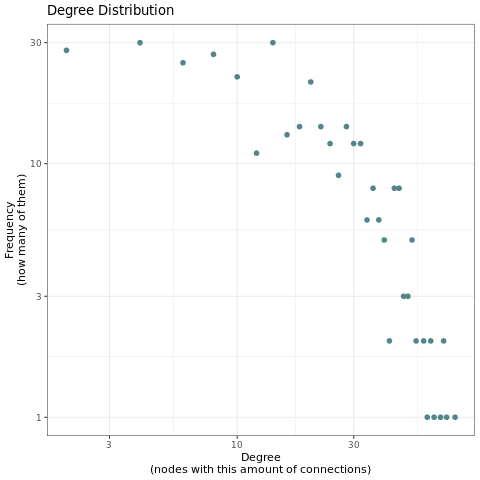
\includegraphics[width=70mm,scale=1.2]{report/figures/degree_distribution.png}

\caption{\textit{Distribución del grado en escala logarítmica}}

\end{center}

En este caso, el coeficiente medio de clustering de nuestra red es de 0.43.
En la figura podemos observar que los nodos con un grado menor varían mucho en cuanto a C, teniendo nodos que están muy agregados y otros que están casi desconectados. 
Esto no pasa en los hubs, que se mantienen muy cercanos en cuanto a transitividad

\begin{center}

\includegraphics[width=70mm,scale=1.2]{report/figures/clustering_coefficient.png}

\caption{\textit{Coeficiente de clustering}}

\end{center}

Si nos fijamos en la distancia entre los nodos de nuestra red, podemos comprobar que tiene propiedad de mundo pequeño, ya que la mayoría de nodos tienen distancia 3 o 4, 
siendo la media 3.46.
Es decir, nuestra red está bien comunicada.

\begin{center}

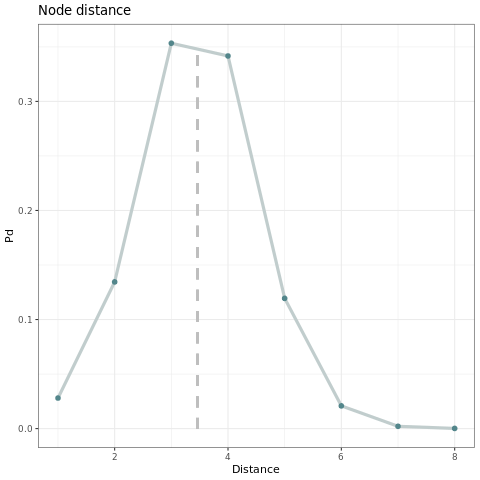
\includegraphics[width=70mm,scale=1.2]{report/figures/Node_distance.png}

\caption{\textit{Distancia entre los nodos}}

\end{center}

En la siguiente figura observamos que la red es bastante robusta ante ataques aleatorios y bastante menos ante ataques dirigidos, lo que nos indica una vez más que el modelo
libre de escala es el que se ajusta mejor.

Que disminuya tan rápido la conectividad eliminando una fracción tan pequeña de nos indica que debemos centrarnos en el estudio de esas proteínas principalmente.

\begin{center}

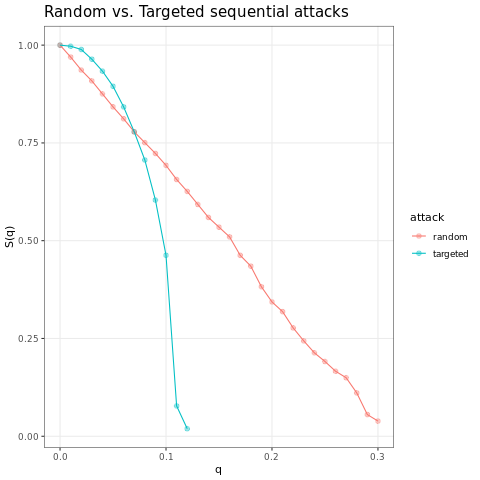
\includegraphics[width=70mm,scale=1.2]{report/figures/sequential_attacks.png}

\caption{\textit{Robustez frente a ataques dirigidos y aleatorios}}

\end{center}

\subsection{Linked Communities}
En esta sección procedemos a obtener las comunidades existentes dentro de nuestra red de proteínas, obtenida en la sección anterior.

Antes debemos tener claro que las comunidades son conjuntos de nodos relacionados entre sí que poseen funciones semejantes y que buscan conseguir un objetivo común. 
Es por ello por lo que la identificación de las comunidades es un problema relevante para muchas áreas de investigación como la sociología, la biología o la informática.

En general, la comunidades se pueden clasificar en dos tipos, las que están formadas por nodos y las que están formadas por enlaces.

\begin{itemize}
\item Comunidad de nodos: Se tratan de subgrafos formados por nodos densamente conectados entre ellos, pero muy poco conectados con los nodos de alrededor, 
como se muestra en la imagen. 


\begin{center}

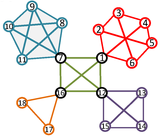
\includegraphics[width=70mm,scale=1.2]{report/figures/nodes.png}

\caption{\textit{Comunidad de nodos}}

\end{center}


\item Link community: Consiste en un subgrafo en el que existe una gran cantidad de enlaces pero muy pocos con las comunidades externas. 
La forma de detectar estos conjuntos es mediante la división de los enlaces de la red. En estas particiones, las conexiones determinan una comunidad, 
pero los nodos pueden pertenecer a varias comunidades. 


\begin{center}
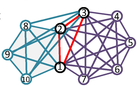
\includegraphics[width=70mm,scale=1.2]{report/figures/links.png}


\caption{\textit{Link community}}

\end{center}

Con esto queremos remarcar que la importancia de la detección de estos subgrafos se debe a que en el campo de la biología, permiten encontrar módulos proteicos con una misma
función celular o predecir las funciones de las proteínas.

Por tanto, diseñaremos un código en R que nos permite la detección de las comunidades con el fin de filtrar aquellas que son más importantes (centralidad). De esta forma,
podemos llevar a cabo un enriquecimiento funcional de las mismas y así obtener algunas de las funciones celulares que determinan red del SARS-CoV-2.

Además, en el código siguiente se incluyen diferentes gráficas para la visualización de las comunidades.
\end{itemize}

A lo largo de la ejecución del código hemos añadido distintas gráficas para la representación de las comunidades. A continuación se muestra un dendograma de las 
\textit{link communities}, en el que se puede apreciar una gran cantidad de comunidades. En esta imagen es difícil ver la centralidad de las comunidades, 
por lo que haremos más representaciones.

\begin{lstlisting}
#link communities dendogram
png(file="linkcomm_dend.png")
plot(proteins.mapped.network.lc, type = "dend")
dev.off()
\end{lstlisting}

\begin{center}
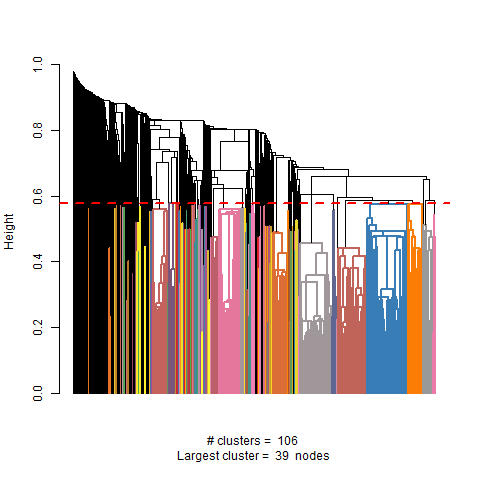
\includegraphics[width=90mm,scale=1]{report/figures/linkcomm_dend.png}


\caption{\textit{Dendograma de Linked Communities}}

\end{center}


Empleando el diseño \textbf{ Fruchterman Reingold} se puede obtener una visión más amplia de las comunidades. 

\begin{lstlisting}
#link communities Fruchterman Reingold layout
png(file="linkcomm_layout.fruchterman.reingold.png")
plot(proteins.mapped.network.lc, type = "graph", layout =
layout.fruchterman.reingold, vlabel=FALSE)
dev.off()
\end{lstlisting}

\begin{center}

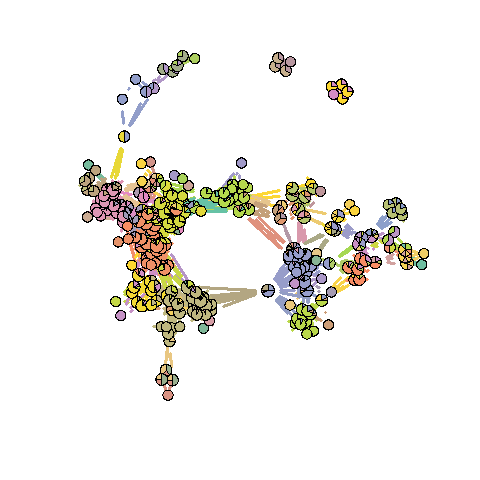
\includegraphics[width=90mm,scale=1]{report/figures/linkcomm_layout.fruchterman.reingold.png}


\caption{\textit{Linked Communities con Fruchterman Reingold layout }}

\end{center}

Sin embargo, lo que nos interesa en este caso es obtener la \textbf{'centralidad comunitaria'} pues se define como la suma de las áreas con mayor influencia sobre los nodos vecinos de la red. Por tanto, nos permite obtener aquellos clusters que ejercen una mayor influencia sobre la red, pudiendo ser determinantes en la funcionalidad de la misma.

Por otra parte, la \textbf{modularidad} consiste en el grado de separación y recombinación existente entre los componentes de una red. Es decir, se considera como una medida de la presencia de estructura comunitaria. Esto permite la búsqueda de comunidades, quedándonos con aquellas que tengan un valor de modularidad positivo y lo más grande posible (modularidad optimizada).

Por ello, hemos calculado la modularidad de las comunidades de nuestra red y hemos representado el valor de la modularidad para cada una de ellas.

\begin{lstlisting}
# Community centrality
community.centrality <- getCommunityCentrality(proteins.mapped.network.lc)

#modularity of the communities
community.connectedness <- getCommunityConnectedness(
proteins.mapped.network.lc,conn = "modularity") 

png(file="communities_modularity.png")
plot(proteins.mapped.network.lc, type = "commsumm", summary = "modularity")
dev.off()
\end{lstlisting}
\begin{center}
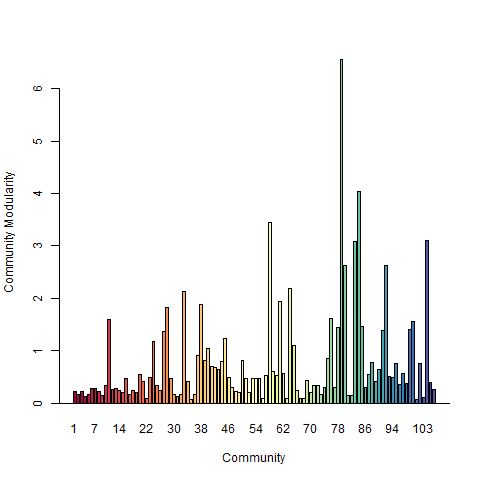
\includegraphics[width=90mm,scale=1]{report/figures/communities_modularity.png}

\caption{\textit{Diagrama de barras de la modularidad de las comunidades}}

\end{center}
En la imagen se observa claramente como hay una comunidad con una modularidad muy alta, lo que indica que esta es más influyente en la red que el resto, concretamente la comunidad 79.


\begin{lstlisting}
# Focus on one linkcomm
#plot one cluster with maximun community modularity
png(file="cluster12_graph.png")
plot(proteins.mapped.network.lc, type = "graph", clusterids =
community.connectedness.maximum, vlabel=FALSE)
dev.off()

\end{lstlisting}

\begin{center}
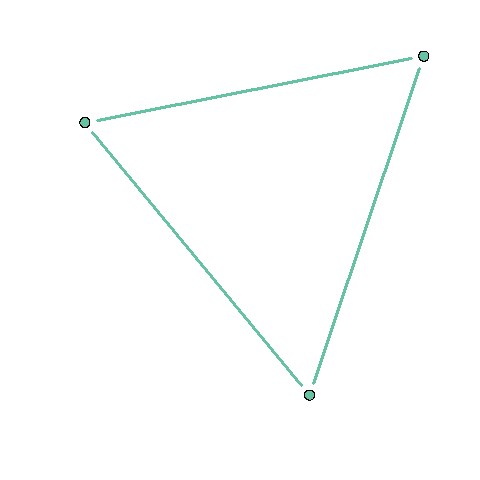
\includegraphics[width=70mm,scale=1]{report/figures/cluster_graph.png}
\end{center}

Por tanto, realizaremos un análisis funcional centrándonos en aquellas comunidades con una modularidad mayor, para determinar si sus funciones moleculares son determinantes o no.

\subsection{Enriquecimiento funcional}
\subsubsection{Cluster 104}

\begin{center}
\vspace{1.5ex}
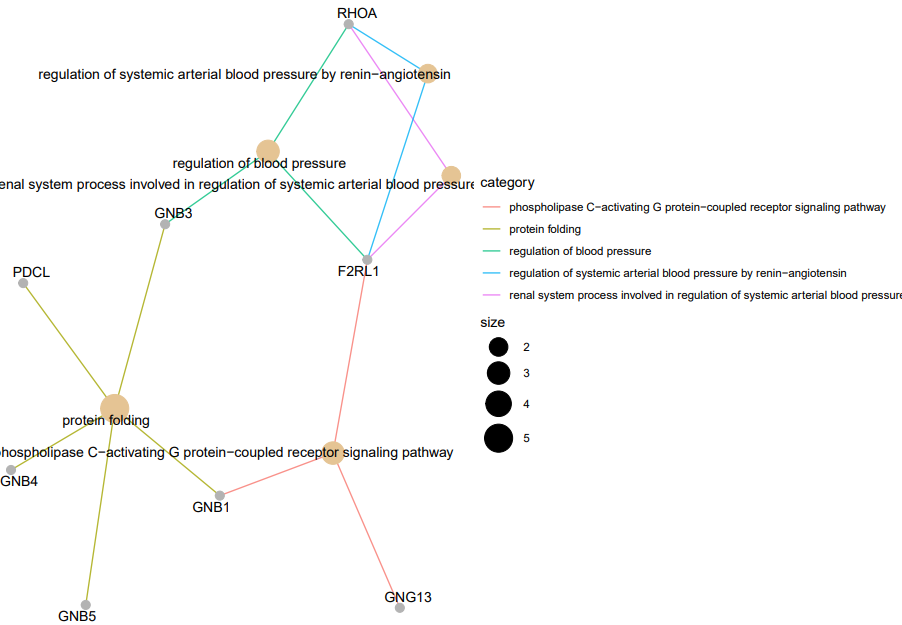
\includegraphics[width=100mm,scale=1.1]{report/figures/enrichGO_heatmap_cnetplot-BP-104-2.PNG}
\vspace{1.5ex}
\end{center}


En la figura superior podemos observar mediante un mapa de calor o heatmap, los 5 términos de la GO predominantes de la subred, además de otras funciones asociadas a cada proteína. 
Para el clúster 104 vemos que el término con un mayor tamaño en el mapa es ‘protein folding’. Esto indica que su GeneRatio (porcentaje de DEGs asociado al término) es grande y el q valor o p valor ajustado, es pequeño.


\begin{center}
\vspace{1.5ex}
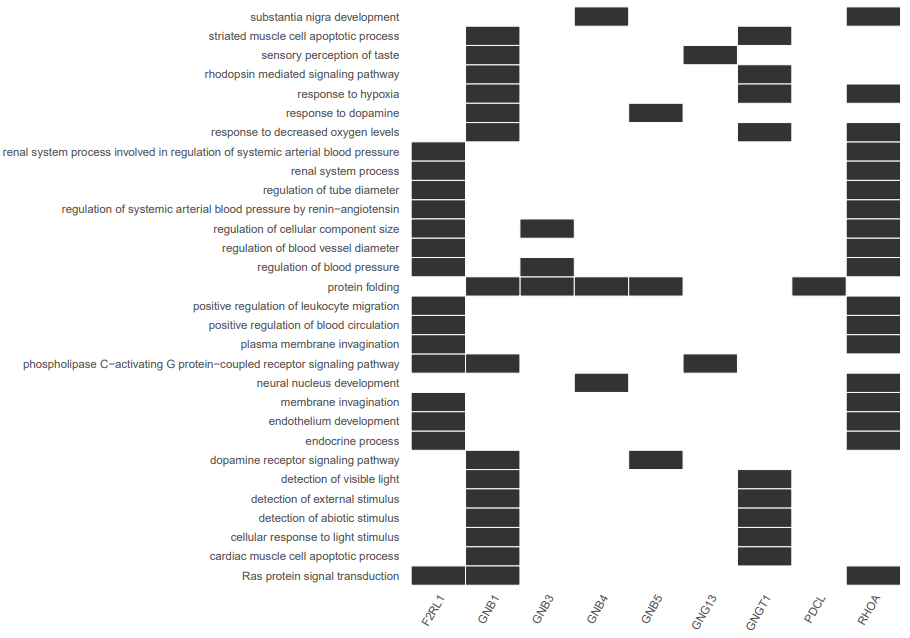
\includegraphics[width=100mm,scale=1.1]{report/figures/enrichGO_heatmap_cnetplot-BP-104-1.PNG}
\vspace{1.5ex}
\end{center}


Investigando en la ontología, obtenemos que el \textbf{plegamiento de proteínas} es un proceso biológico que facilita el ensamblaje de proteínas para dar lugar a una estructura terciaria correcta.


De ahí podemos deducir el papel que juega esta función pues un fallo en plegamiento puede provocar un desorden celular con amplias consecuencias. Es más, existen una gran cantidad de enfermedades generadas por este tipo de fallos como el Alzheimer, el Parkinson, la fibrosis quística y muchos otros trastornos degenerativos, tal y como se mencionan en el artículo \textbf{\textit{‘Protein-misfolding diseases and chaperone-based therapeutic approaches’}}.
Según este estudio, “más de la mitad de las enfermedades humanas podrían estar relacionadas con un plegamiento incorrecto de las proteínas”. Este proceso parece afectar a las chaperonas, pues son las encargadas de reparar las mutaciones que causan las patologías.

Por otra parte, la \textbf{‘ruta de señalización del receptor acoplado a la proteína G que inhibe la fosfolipasa C’}, es otro de los procedimientos identificados en mayor medida con el clúster en cuestión.   Concretamente, esta vía además de inhibir la actividad de la fosfolipasa C, conlleva una disminución de los niveles de DAG y IP3. Este último es un mensajero de señalización celular cuya disminución parece estar relacionada con la \textbf{autofagia} o vía de degradación de proteínas, orgánulos y material citoplasmático. Por su parte, los segundos mensajeros DAG dan lugar a la activación de la proteína quinasa C, la cual permite la activación de una serie de rutas metabólicas que inducen la expresión de proteínas que activan los linfocitos T. Estos desempeñan un papel fundamental en la regulación del sistema inmune, por lo que una alteración de los mismo puede generar una inmunodeficiencia severa.

\begin{center}
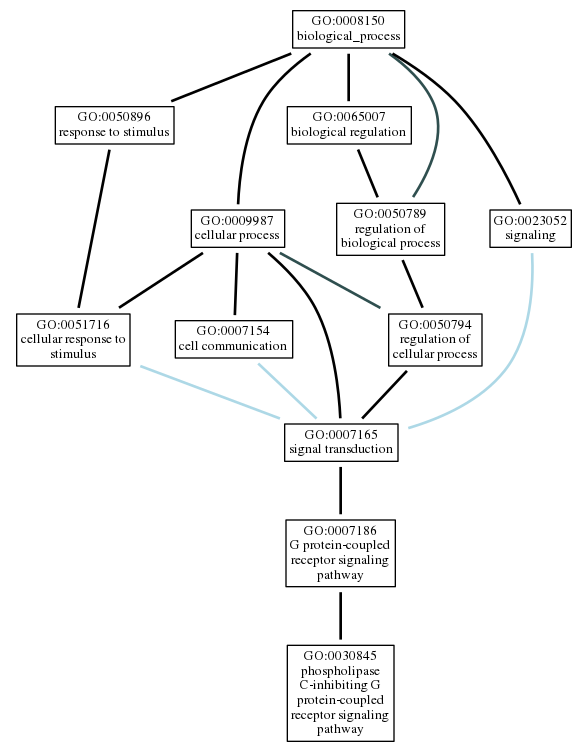
\includegraphics[width=70mm,scale=1]{report/figures/signaling pathway.png}
\end{center}

Otra de las funciones biológicas que aparecen en el enriquecimiento de este módulo, está relacionada con la \textbf{regulación de la presión sanguínea}, y, por tanto, de los niveles de oxígeno. Este es un proceso muy complejo que viene determinado por el Sistema Nervioso Autónomo, el SNC y el riñón. El objetivo del SN es mantener la presión arterial (PA) mediante la regulación de los niveles de oxígeno. Sin embargo, un nivel alto de PA o \textbf{hipertensión}, puede llegar a ser nocivo para el corazón, puesto que lo obliga a bombear más sangre, contribuyendo así al endurecimiento de las arterias, a la producción de accidentes cerebrovasculares, enfermedades renales o insuficiencia cardíaca.

Según un estudio reciente, \textbf{\textit{'COVID-19 and Hypertension: What We Know and Don't Know'}}, el SARS-CV-2 interactúa con el Sistema renina-angiotensina aldosterona (RAAS), actuando sobre el receptor ACE2 induciendo una desregulación de la misma, lo que genera la acumulación lo local de angiotensina II.  Debido a que el sistema RAAS se encarga de regular la presión arterial, la alteración del mismo da lugar a la hipertensión de los pacientes.

\begin{center}
\vspace{1ex}
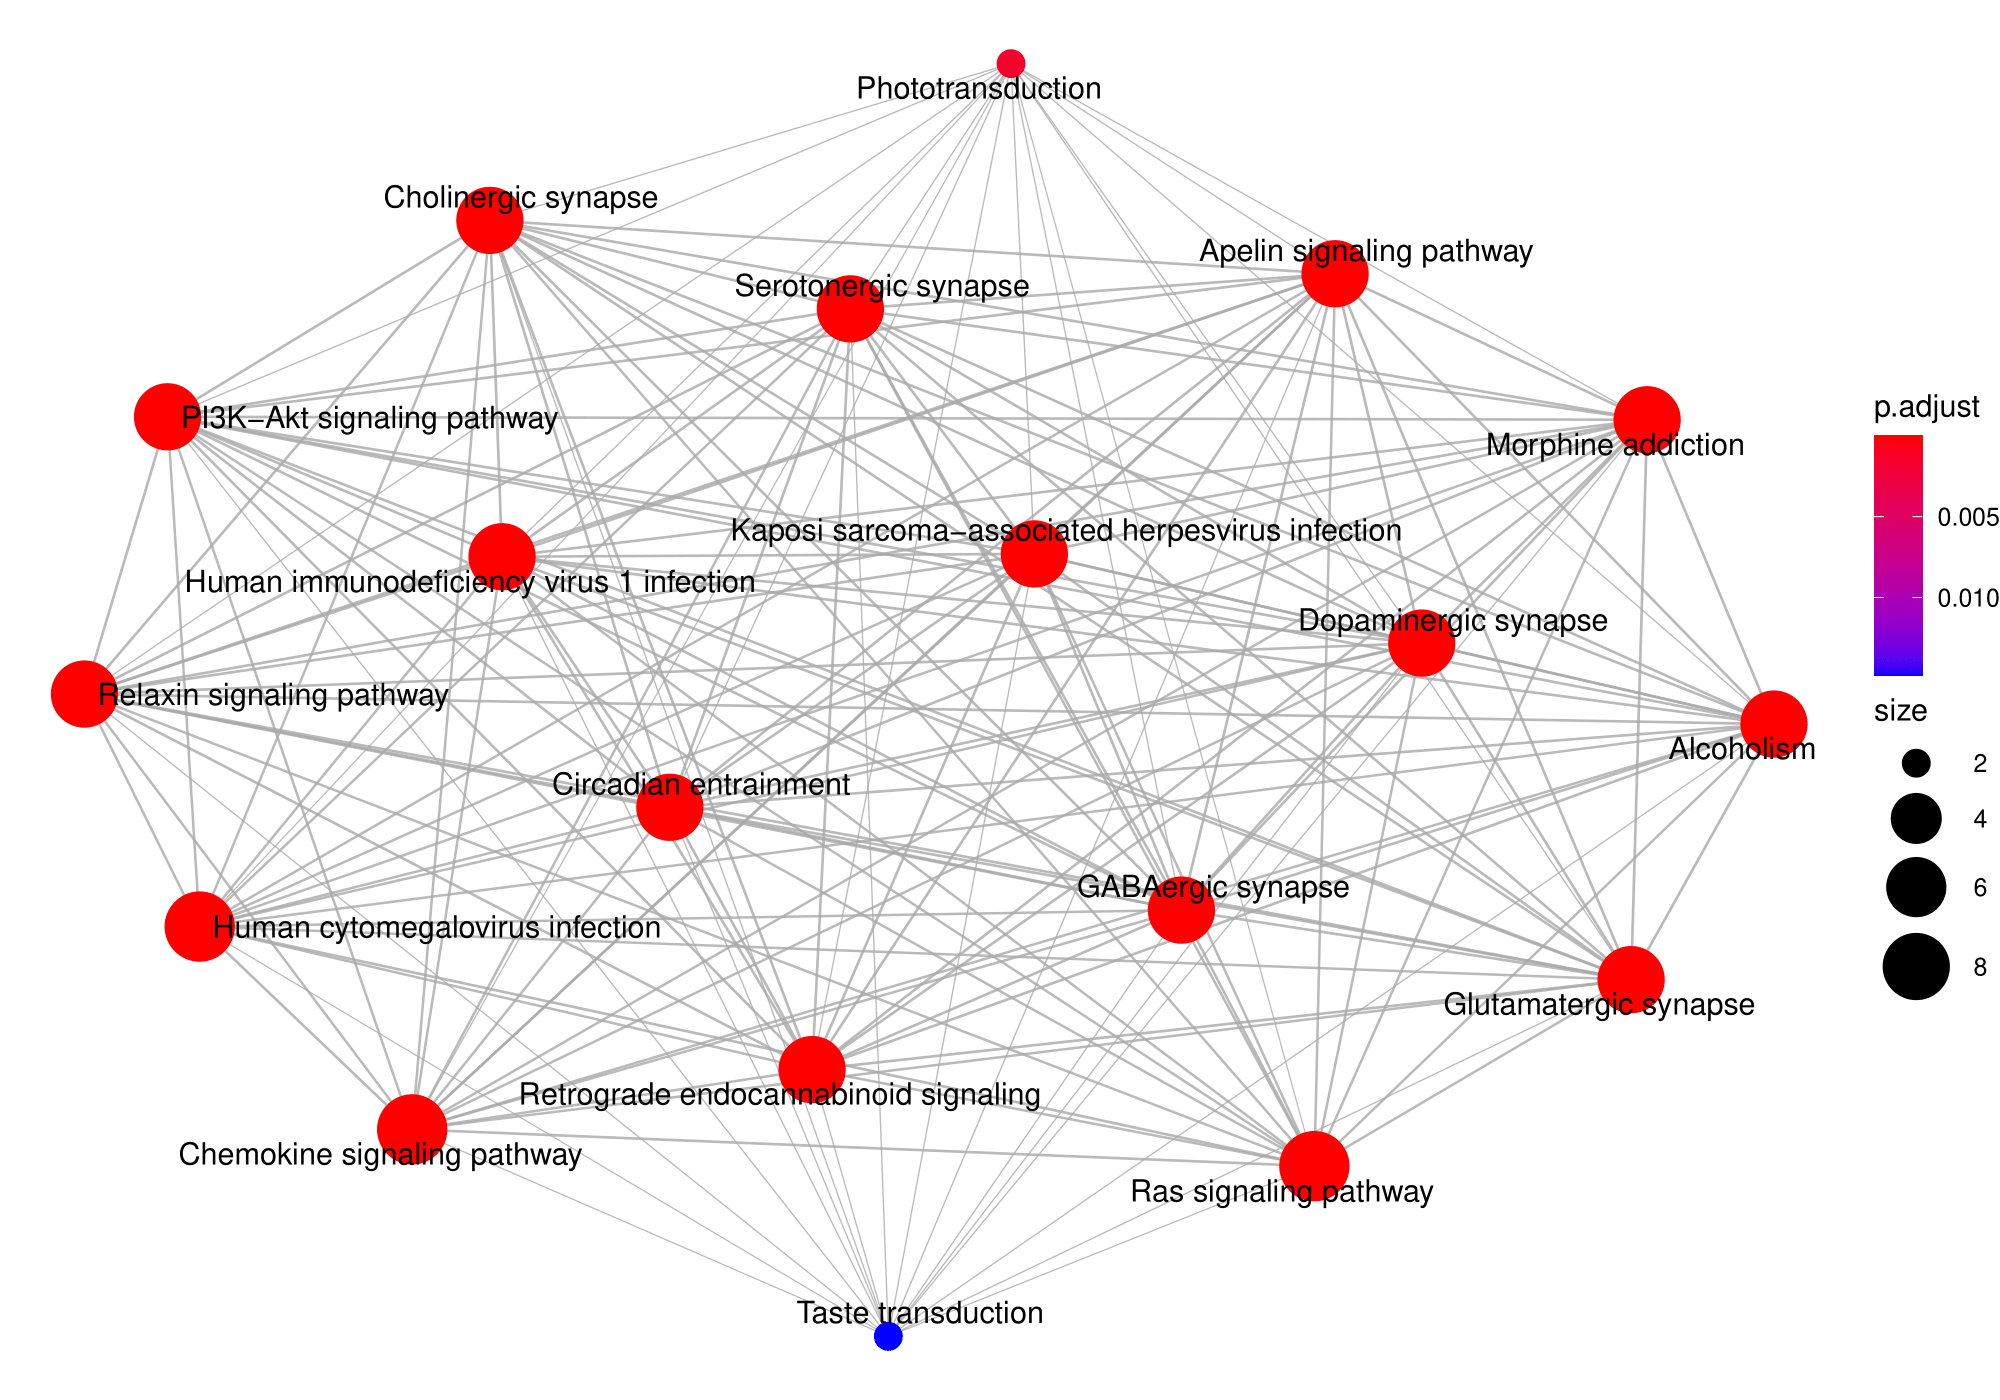
\includegraphics[width=100mm,scale=1]{report/figures/enrichKEGG_enrichmap-BP-104.png}
\vspace{1ex}
\end{center}

Para concluir, en la figura superior podemos observar como alguno de los procesos mencionados se encuentran en el mapa de vías metabólicas. Además, en el mapa de calor obtenido, también se observan muchos de los términos más presentados en el clúster 104.

\subsubsection{Clúster 84}

\begin{center}
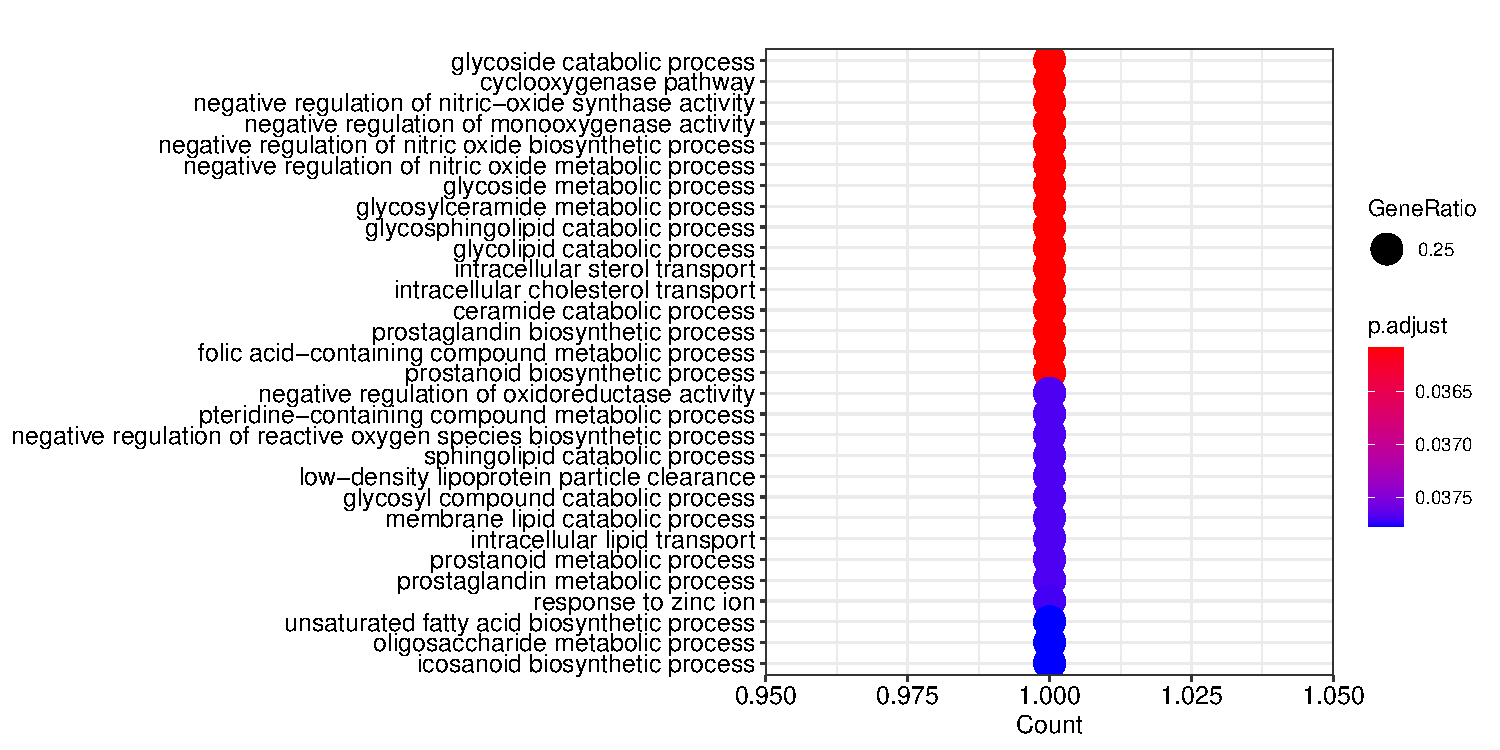
\includegraphics[width=120mm,scale=1]{report/figures/enrichGO_dotplot-BP-84.pdf}
\end{center}

Este clúster está formado por 4 proteínas altamente interconectadas cuyas funciones biológicas se relacionan con 4 aspectos principalmente. El primero de ellos y el más abundante es el \textbf{metabolismo y catabolismo de glúcidos y lípidos}, los cuales son nuestra principal fuente de energía en el organismo. El hecho de que las proteínas del virus interactúen con las de nuestro clúster puede provocar alteraciones en el desarrollo de esta función tan esencial. El siguiente tema a tratar es la \textbf{regulación negativa del óxido nítrico}. Este compuesto es mencionado en varias de las funciones biológicas de nuestras proteínas y se trata de un gas que se genera en el endotelio. Se caracteriza por tener propiedades vasodilatadoras y contribuir al mantenimiento de la presión arterial baja. Por tanto, una regulación negativa del mismo significaría un déficit de este gas en el cuerpo, lo que puede producir entre otras cosas, hipertensión arterial. En tercer lugar en nuestras funciones se hace mención a la \textbf{ruta de la ciclooxigenasa (COX)} y por tanto a sus principales productos que son las \textbf{prostaglandinas}. Éstas son un conjunto de sustancias de carácter lipídico derivadas de los ácidos grasos que conllevan diversos efectos en nuestro organismo, a menudo contrapuestos. Las prostaglandinas afectan y actúan sobre diferentes sistemas, incluyendo el sistema nervioso, el músculo liso y el sistema reproductor. Además, juegan un papel importante en regular diversas funciones como la presión sanguínea, la coagulación de la sangre, la respuesta inflamatoria alérgica y la actividad del aparato digestivo. Por tanto, la interacción del virus con estos compuestos pueden suponer un ataque en nuestro cuerpo. Finalmente aparecen varias funciones relacionadas con el \textbf{transporte intracelular}, lo cual es de vital importancia en las células para expulsar de su interior los desechos del metabolismo o trasladar sustancias que sintetiza como hormonas entre otras actividades.

\begin{center}
\vspace{1.5ex}
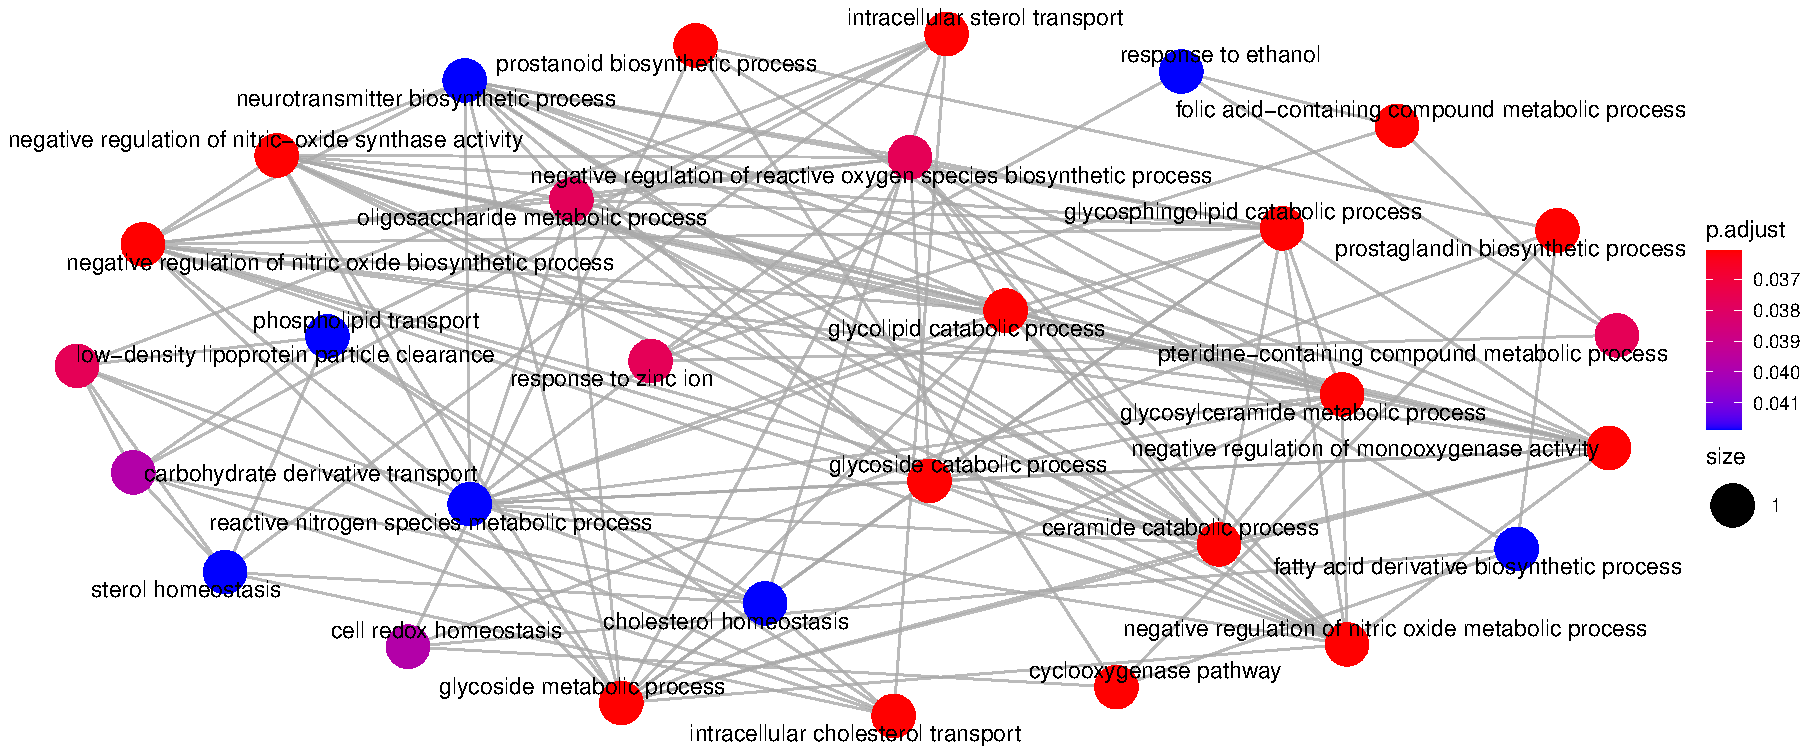
\includegraphics[width=100mm,scale=1]{report/figures/enrichGO_enrichmap-BP-84.pdf}
\vspace{1.5ex}
\end{center}

Además, se puede apreciar como la clasificación de nuestras funciones en estos 4 aspectos se encuentra claramente reflejada en la figura anterior, donde las proteínas pertenecientes a un mismo tema presentan un mayor número de conexiones entre ellas.

\subsubsection{Clúster 79}
La principal funcionalidad que podemos ver es la biosíntesis de las proteínas de membrana GPI: Proteínas de la superficie celular que se pueden unir a la membrana mediante una estructura de glicolípidos denominadas \textbf{anclaje de glicosilfosfatidilinositol (GPI)}. Las proteínas que son detectadas en el cluster con una mayor fiabilidad estadística son las necesarias para la construcción de estas estructuras. Procesos celulares asociados a la biosíntesis de lipoproteínas son atribuidos a dichas proteínas junto con procesos metabólicos de la formación de estos complejos GPI. 

\begin{center}
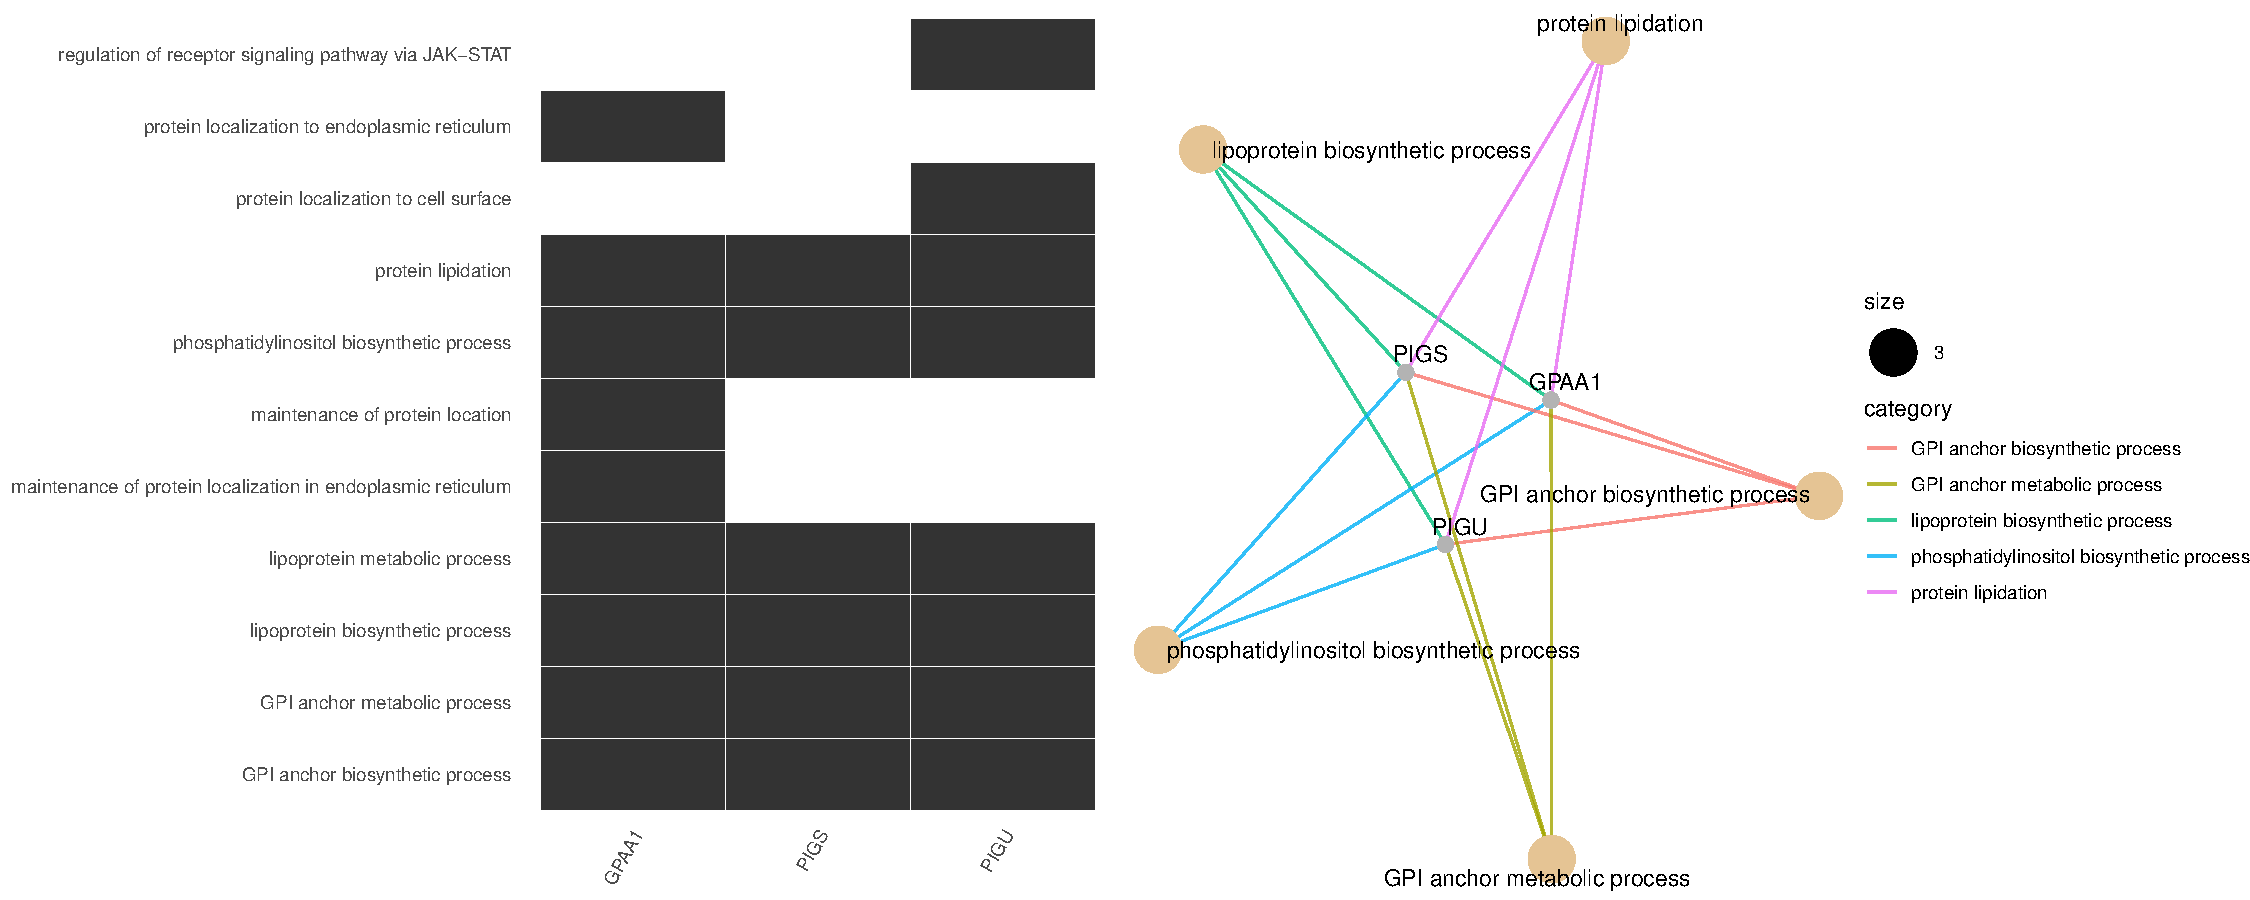
\includegraphics[width=100mm,scale=1.1]{report/figures/enrichGO_heatmap_cnetplot-BP-79.pdf}
\end{center}
\vspace{1.5ex}


Estas estructuras conforman las balsas lipídicas en las membranas celulares las cuales son zonas accedidas por ciertas proteínas del SARS-CoV2, en concreto la proteína \textbf{ORF9c}, la cual podría tratarse de una de las proteínas del coronavirus humano que adquiere un dominio de transmembrana mediante la interacción con estos anclajes y que podría estar asociada con el ataque hacia procesos de señalización inmunológicos. En recientes estudios se muestra cómo ORF9c interactúa con las proteínas de membrana y altera los procesos antivirales en líneas celulares epiteliales pulmonares.

Además se observa que estos componentes son incluso mecanismo de entrada directa en otros virus y se aprecian diferencias en cuanto a estos procedimientos en distintos tipos de coronavirus.

\vspace{1.5ex}
\begin{center}
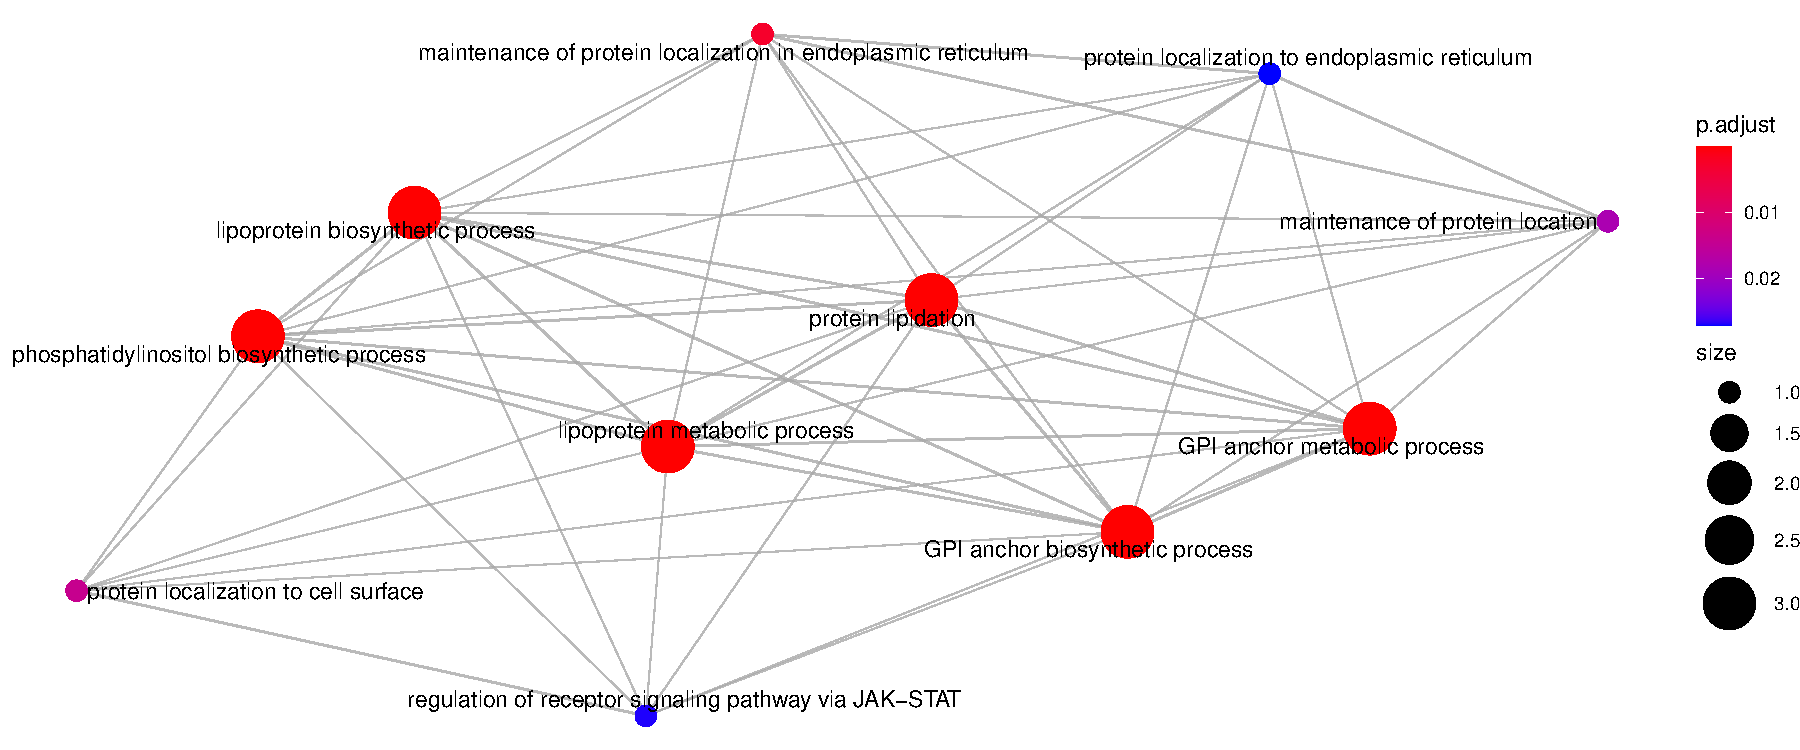
\includegraphics[width=100mm,scale=1.1]{report/figures/enrichGO_enrich_map-BP-79.pdf}
\end{center}
\vspace{1.5ex}

En este caso nuestro análisis de las comunidades proteicas nos ha llevado a concretar la importancia funcional que podría ayudar a estudiar más en profundidad la acción del SARS-CoV2 a partir de un nivel topológico. 

\subsubsection{Clúster 58}

\begin{center}
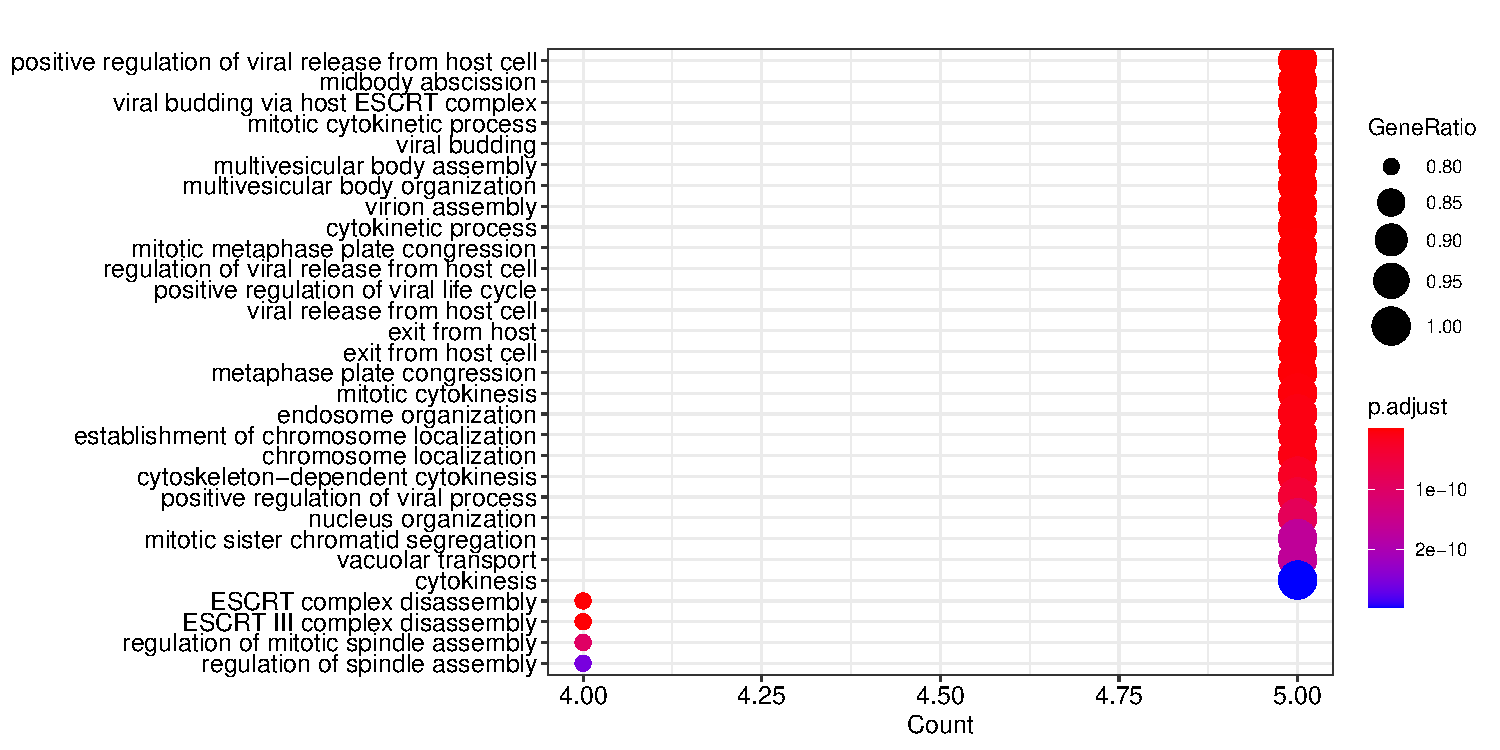
\includegraphics[width=120mm,scale=1]{report/figures/enrichGO_dotplot-BP-58.pdf}
\end{center}

Este grupo de 5 proteínas es sin duda el más interesante para nuestro estudio. Sus funciones están altamente vinculadas a la actividad viral en nuestro organismo, lo que ya explica de entrada el motivo de su interacción con las proteínas del covid. Tras la detenida lectura de todas sus funciones se pueden extraer una serie de elementos fundamentales que aparecen en repetidas ocasiones. A continuación, muestro una breve explicación de las más relevantes:

\begin{enumerate}
    \item \textbf{Liberación viral de la célula huésped}: Esta función biológica se asocia con la replicación de los virus en nuestro organismo, de tal forma que permite la salida de viriones de una célula infectada para promover la propagación del virus de célula a célula. Una vez ensambladas en el sitio de replicación, las partículas virales pueden liberarse por gemación, exocitosis, extrusión o lisis de la célula huésped. Algunos virus también median el transporte directo de su genoma viral a las células adyacentes gracias a las proteínas de movimiento. 
    \item \textbf{Incipiente viral}: Proceso viral mediante el cual los virus envueltos adquieren una membrana derivada del hospedador enriquecida en proteínas virales para formar su envoltura externa. El proceso comienza cuando las nucleocápsidas, ensambladas o en proceso de construcción, inducen la formación de una curvatura de la membrana en el plasma del huésped o la membrana del orgánulo y se envuelven en la yema en formación. El proceso termina cuando la yema es finalmente pellizcada por la escisión de la membrana para liberar la partícula envuelta en el espacio lumenal o extracelular.
    \item \textbf{Ensamblaje del cuerpo medio y citocinesis}: La citocinesis consiste en la separación física del citoplasma en dos células hijas durante la división celular. El cuerpo medio es una estructura transitoria que conecta a ambas células al final de este proceso con la función principal de localizar el sitio de abscisión que separa físicamente a las dos. 
    \item \textbf{Cuerpos multivesiculares}: Tipo especial de lisosoma recubierto por una membrana que contiene en su interior un variable número de pequeñas vesículas. Estos cuerpos también se denominan endosomas tardíos y son la antesala de la degradación de las moléculas endocitadas, la cual se realiza finalmente en los lisosomas gracias a unas enzimas denominadas hidrolasas ácidas.
\end{enumerate}

\begin{center}
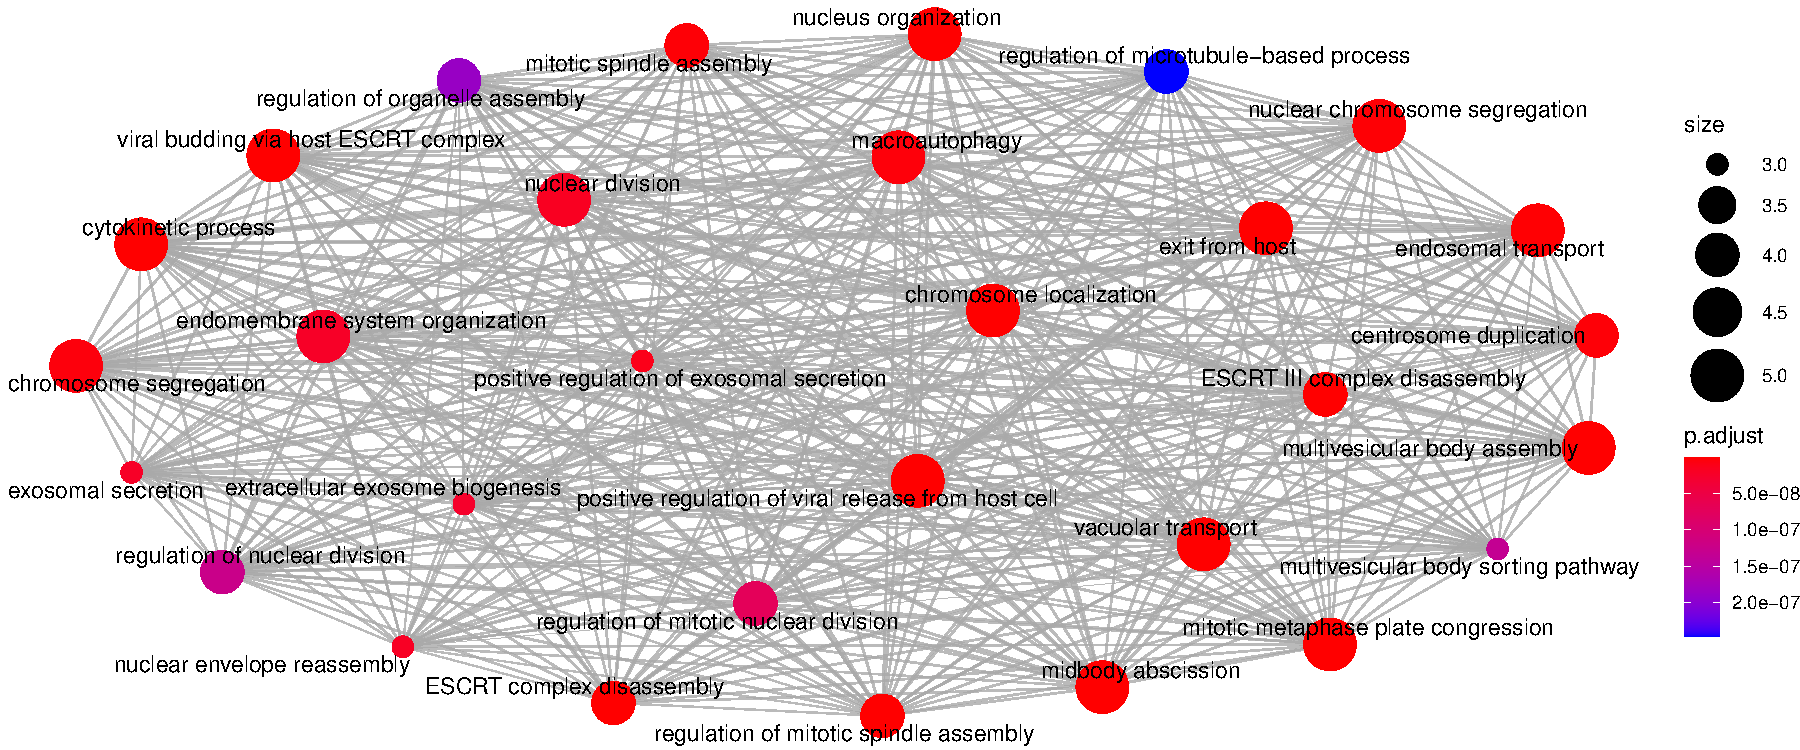
\includegraphics[width=100mm,scale=1]{report/figures/enrichGO_enrichmap-BP-58.pdf}
\end{center}

Las fuertes conexiones entres estos conceptos y la interacción del covid en nuestro organismo son evidentes. Además, cabe destacar el hecho de que las funciones de este clúster presentan grandes vínculos entre sí. Son funciones extremadamente relacionadas que comparten un mismo fin o que participan en localizaciones y lapsos de tiempo muy cercanos. Es por esto que la red presentada en la figura anterior muestra una gran cantidad de enlaces donde todos los nodos poseen un grado bastante elevado.

\subsection{Búsqueda en Drugbank}

La búsqueda en drugbank arroja los siguientes resultados:

\begin{lstlisting}

IDs de los medicamentos cuyos targets se encuentran entre las
proteínas más conectadas de la red  DB00753; DB01189 DB01133 
DB03147 DB05015; DB06603 DB00175; DB00227; DB00277; DB00313;
DB00641; DB01076; DB01095; DB01223; DB01303; DB02546; DB06176;
DB09091 DB00157 DB12010 DB00570
\end{lstlisting}

A continuación, analizaremos algunos de ellos.\newline


\begin{itemize}
    \item \underline{Enfermedades cardiovasculares}
\end{itemize}


\subsubsection{Pravastatin, Lovastatin}

La pravastatina es un medicamento que se suele usar para tratar y prevenir los eventos coronarios, disminuyendo la mortalidad en caso de que estos se den.


\begin{center}

\includegraphics[width=100mm,scale=1]{report/figures/pravastatina.PNG}

\caption{\textit{Ruta metabólica de la pravastatina }}

\end{center}

 Existen evidencias de que el SARS-Cov-2 puede afectar al corazón\cite{Oudit2009SARS-coronavirusSARS}, agravando la condición de los pacientes y dejando secuelas que podrían ser
 de por vida, por lo que el tratamientos de estos eventos coronarios y su prevención podría ser clave para reducir la mortalidad y mejorar la calidad de vida del enfermo.

\subsubsection{Atorvastatin, Rosuvastatin, Fluvastatin, Simvastatin}

\begin{center}
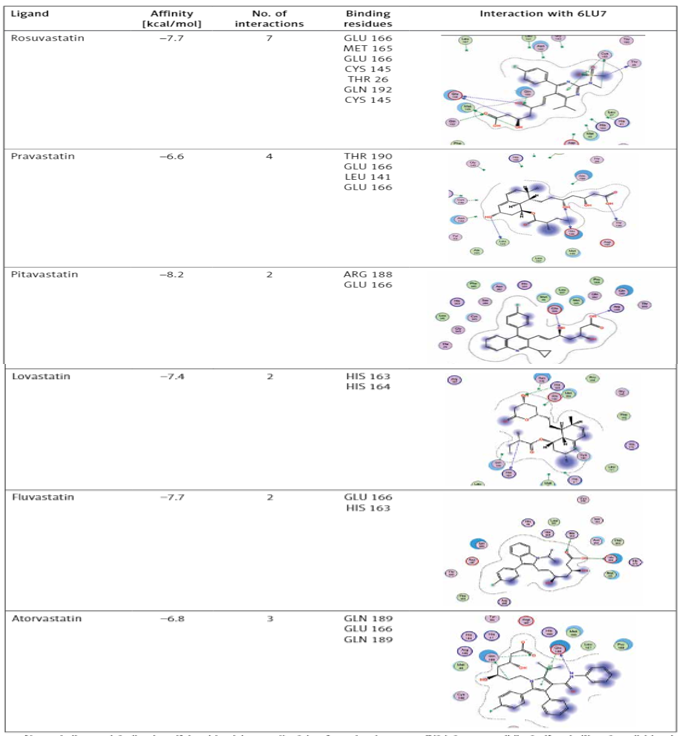
\includegraphics[width=100mm,scale=1]{report/figures/statins.PNG}


\caption{\textit{Tabla de afinidad de las estatinas tomada de \cite{Reiner2020StatinsInteraction} }}
\end{center}

Las \textbf{estatinas o statins} son una clase de medicamento que se emplean para el tratamiento de la dislipemia, concentración elevada lípidos o baja en lipoproteínas. En
concreto, es son medicamentos muy usados para tratar las enfermedades cardiovasculares (ECV) como la aterosclerosis o la angina, puesto que los niveles elevados de colesterol
(LDL) suponen un gran riesgo en el desarrollo de estas enfermedades, y este tipo de medicamentos dan lugar a una reducción significativa  de los niveles de LDL.

Además, en el artículo \textbf{\textit{'Statins and the COVID-19 main protease: in silico evidence on direct interaction' }}se llegó a la conclusión de que las estatinas podrían
ser inhibidores eficaces del SARS-CoV-2. Por tanto al igual que la pravastatina, cualquiera de estos medicamentos podrían ser útiles para la lucha contra el Covid-19, y más
específicamente, contra los efectos cardíacos que provoca.\newline

\begin{itemize}
    \item \underline{Enfermedades respiratorias}
\end{itemize}


\subsubsection{Theophylline, Oxtriphylline}

Medicamentos como la teofilina o oxtrifilina están indicados para tratar los síntomas de asma y bronquitis, entre otras patologías.
Dado que comparten algunos síntomas en común con nuestro caso de estudio, este tipo de medicamentos podrían ser útiles para su tratamiento.

\begin{center}

\includegraphics[width=90mm,scale=1]{report/figures/adenosine.PNG}


\caption{\textit{Vista 3D del receptor A2A adenosina}}

\end{center}

En el caso de la oxtrifilina, se trata de un broncodilatador cuyo mecanismo de acción implica al recepto A2A adenosina, que ya se había propuesto como sujeto de estudio.
\cite{Abouelkhair2020TargetingHypothesis}

\subsubsection{Aminophylline}

La aminofilina es un fármaco formado a partir de teofilina y etilendiamina que es inyectado por vía intravenosa y tiene una gran aplicación para el tratamiento de \textbf{edemas pulmonares} (exceso de líquido en los pulmones). Su mecanismo de acción consiste en libera la teofilina que actúa relajando el músculo liso (broncodilatación) y suprimiendo las respuestas de las vías respiratorias a los estímulos. Estos resultados sobre el organismo permiten el control de los síntomas y un mejor funcionamiento del sistema respiratorio.

Sin embargo, según estudios recientes, este medicamento provoca diversos efectos adversos provocados por la inhibición de PDE III y  el receptor antagonista de la adenosina, que dan lugar a dolores de cabeza, mareos, vómitos, arritmias, etc. Por tanto, se sugiere el empleo de otros broncodilatadores como los anteriormente mencionados.\newline


\begin{itemize}
    \item \underline{Tratamiento de tumores}
\end{itemize}

\subsection{Panobinostat}

Además del panobiostat, la búsqueda en drugbank muestra varios medicamentos más cuya función principal es el tratamiento de diversos tipos de cánceres.

En este caso, inhibe a las histonas DACs, que son responsables de diversos procesos celulares, entre ellos expresión génica y metabolismo de las proteínas.

Tal y como se describe en \cite{White2021PlitidepsinEEF1A.}\textbf{\textit{'Plitidepsin has potent preclinical efficacy against SARS-CoV-2 by targeting the host protein eEF1A'}}, sería interesante ver como podría aplicarse la acción de este tipo de fármacos al tratamiento del SARS-CoV-2.

\begin{center}

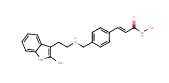
\includegraphics[width=90mm,scale=1]{report/figures/panobiostat.PNG}


\caption{\textit{Estructura molecular del panbiostat}}

\end{center}

\subsection{Belinostat}

El belinostat es un fármaco huérfano relativamente "jóven" que inhibe la enizma histona desacetilasa (HDAC), atacando a \textbf{linfoma de células T periféricas} que ha recidido o que no ha podido ser a tratado con otro tratamiento. Actúa bloqueando la multiplicación celular y destruyendo células cancerosas.
Además, previene el crecimiento de los vasos sanguíneos, impidiendo así el crecimiento del tumor.\newline


\begin{itemize}
    \item \underline{Sedaciónn e intubación}
\end{itemize}

\subsection{Isoflurane, Desflurane}

Normalmente, los pacientes gravemente infectados son sedados e intubados, pero todavía no se están empleando anestésicos volátiles para ello. Sin embargo, se han realizado varios estudios que sugieren que la administración de anestésicos volátiles como el isoflurano o desflurano a pacientes con síndrome de dificultad respiratoria aguda (SDRA), mejora significativamente la oxigenación y el control de la sedación profunda y rápida. Es más, en el estudio \textbf{\textit{'Sevoflurane, a sigh of relief in COVID-19?'}} ha obtenido como resultados que la mortalidad se reduce en un 35 por ciento (confianza del 95 por ciento: 0,18-0,68) en pacientes sedados con isoflurano, en comparación con propofolmidazolam. 

Estos beneficios potenciales se deben principalmente a que los anestésicos volátiles presentan propiedades inmunomoduladoras que reducen las señales de muerte y, por tanto, la respuesta inflamatoria.  Por tanto, el uso de este tipo de fármacos cuyos targets son algunas de las proteínas de nuestra red, podrían contribuir notablemente a la reducción de la lesión pulmonar.


